In this subsection the evaluation of the model trained on ER dataset with stronger regularization is presented. Based on the quantitative metrics of Pearson and Spearman rank correlation coefficients it was concluded that the UNet predictions performance for the ER case if even better than for nuclei. The exact values are presented in Table \ref{table:er-downstream-metrics-coefficients}. Especially the improvement in mean and total intensities correlations is noticable (lower correlation in case of nuclei (see Table \ref{table:nuclei-downstream-metrics-coefficients})). 

The quality of predictions in terms of the number of ER and their area is very good. Both scatter plots confirm this as the line is almost diagonal for both os these metrics. The shapes of the distributions of count and area are very similar as well, which is depicted via the violin plots (see Figure \ref{fig:er-downstream-metrics-2}). For example, the mean values are almost identical (middle line in the box plot inside the violin). 

Visually predictions look slightly brigher, however this difference is less evident after a visual examination in comparison to the nuclei case. Nevertheless, the predictions do tend to have a slightly higher intensities and that was captured in the violin plots (see Figure \ref{fig:er-downstream-metrics-1}), where is it clear that the ER prediction images are brighter. The mean values inside the box plots confirm this observation by being higher for the predictions.

\begin{figure}[htb]
	\begin{center}
		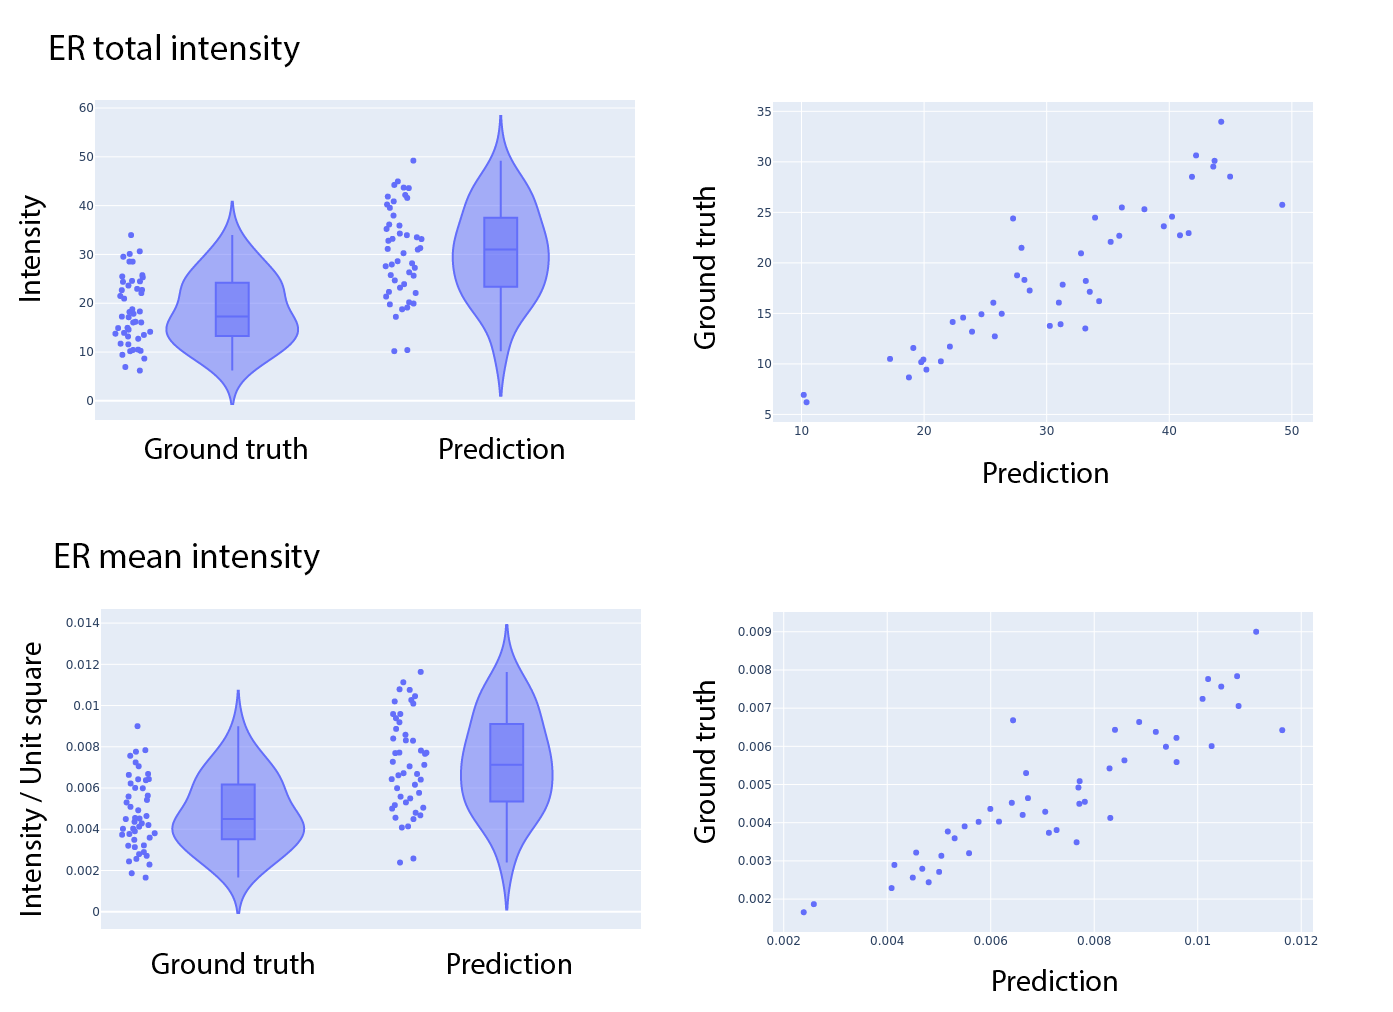
\includegraphics[width=0.8\linewidth]{bilder/ER/metrics/combined-metrics-1.png}
		\caption{Metrics for practical biological evaluation on ER. Total and mean intensities}\label{fig:er-downstream-metrics-1}
	\end{center}
\end{figure}

While nuclei mostly were easily separable, this is not the case in the ER dataset, where several ER can form one bigger region together (see \ref{fig:er-segmentation-steps}.6). In such situation extraction of the intensities metrics from \textit{findContours} method will extract the mean and total intensities of the whole region rather than for separate ERs. Because at the end metrics are averages across every ER in one image, we did not encounter for this fact as there is not a huge difference in the evaluation. However for a more precise evaluation it might be helpful to apply watershed algorithm to separate the ERs first.

\begin{figure}[htb]
	\begin{center}
		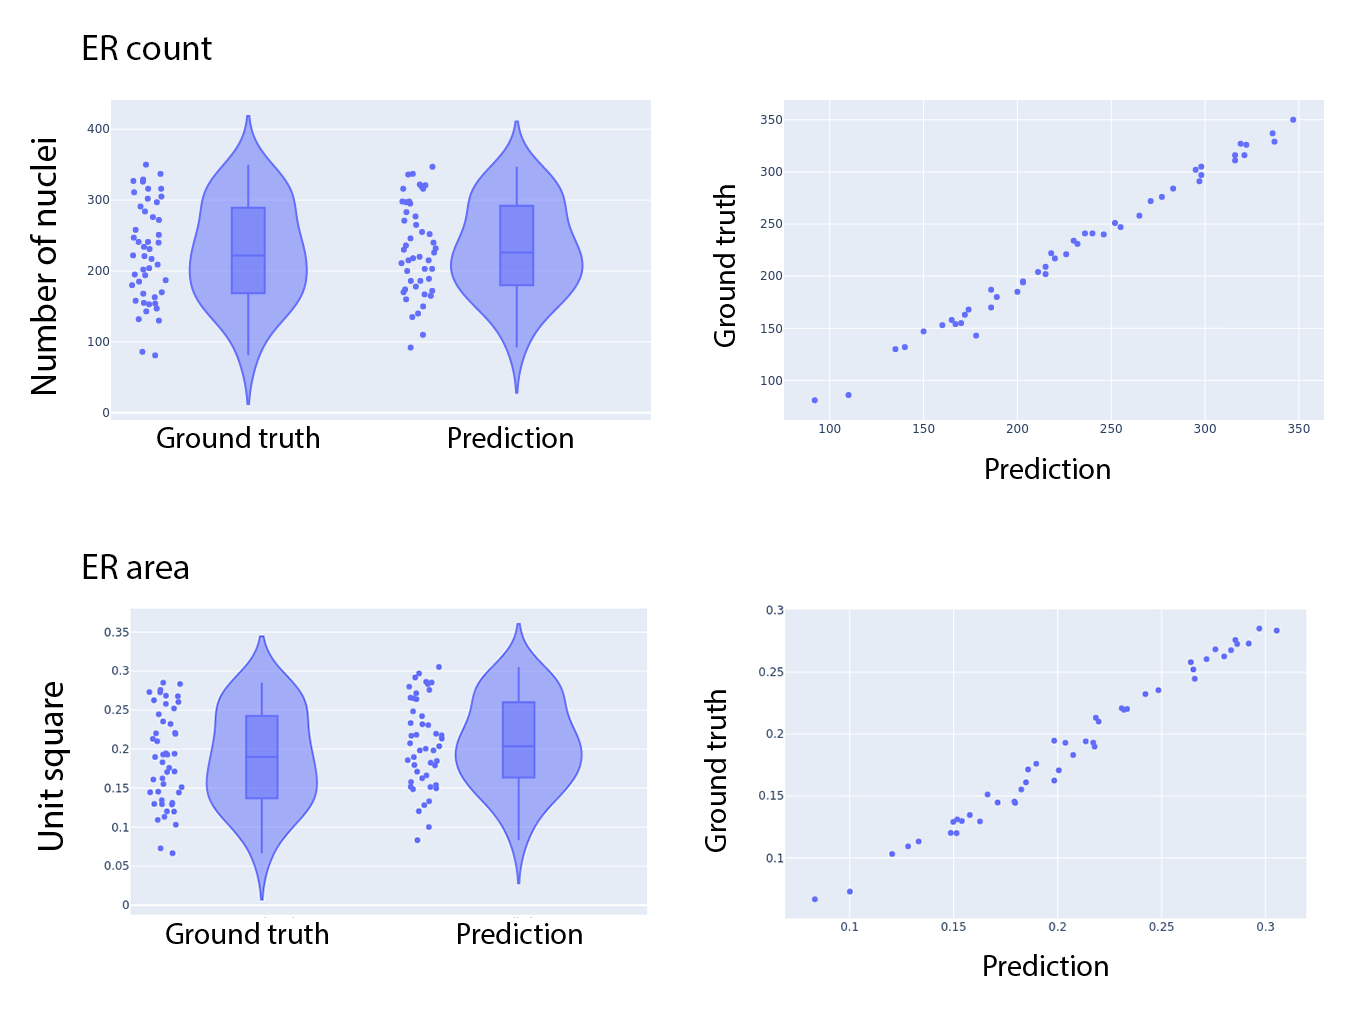
\includegraphics[width=0.8\linewidth]{bilder/ER/metrics/combined-metrics-2.png}
		\caption{Metrics for practical biological evaluation on ER. Count and area}\label{fig:er-downstream-metrics-2}
	\end{center}
\end{figure}

\begin{table}[htb]
    \centering
    \caption{Correlation coefficients for practical biological evaluation on ER}
        \begin{adjustbox}{width=0.4\textwidth}
            \begin{tabular}{|c|c|c|}\hline
                &Pearson&Spearman
                \\\hline\hline
                Number of ER & 0.988 & 0.984\\\hline
                Total intensity&0.952&0.955\\\hline
                Mean intensity&0.941&0.933\\\hline
                Area &0.991&0.990\\\hline
            \end{tabular}
        \label{table:er-downstream-metrics-coefficients}
        \end{adjustbox}
\end{table}
